\documentclass{article}

\usepackage{amsmath,amssymb}
\usepackage{tikz}
\usepackage{pgfplots}
\usepackage{xcolor}
\usepackage[left=2.1cm,right=3.1cm,bottom=3cm,footskip=0.75cm,headsep=0.5cm]{geometry}
\usepackage{enumerate}
\usepackage{enumitem}
\usepackage{marvosym}
\usepackage{tabularx}

\usepackage{listings}
\definecolor{lightlightgray}{rgb}{0.95,0.95,0.95}
\definecolor{lila}{rgb}{0.8,0,0.8}
\definecolor{mygray}{rgb}{0.5,0.5,0.5}
\definecolor{mygreen}{rgb}{0,0.8,0.26}
\lstdefinestyle{java} {language=java}
\lstset{language=java,
	basicstyle=\ttfamily,
	keywordstyle=\color{lila},
	commentstyle=\color{lightgray},
	stringstyle=\color{mygreen}\ttfamily,
	backgroundcolor=\color{white},
	showstringspaces=false,
	numbers=left,
	numbersep=10pt,
	numberstyle=\color{mygray}\ttfamily,
	identifierstyle=\color{blue},
	xleftmargin=.1\textwidth, 
	%xrightmargin=.1\textwidth,
	escapechar=§,
	breaklines=true,
	postbreak=\mbox{\space}
}

\usepackage[utf8]{inputenc}

\renewcommand*{\arraystretch}{1.4}

\newcolumntype{L}[1]{>{\raggedright\arraybackslash}p{#1}}
\newcolumntype{R}[1]{>{\raggedleft\arraybackslash}p{#1}}
\newcolumntype{C}[1]{>{\centering\let\newline\\\arraybackslash\hspace{0pt}}m{#1}}

\newcommand{\E}{\mathbb{E}}
\DeclareMathOperator{\rk}{rk}
\DeclareMathOperator{\Var}{Var}
\DeclareMathOperator{\Cov}{Cov}

\title{\textbf{Softwaretechnologie, Übung 10}}
\author{\textsc{Henry Haustein}}
\date{}

\begin{document}
	\maketitle
	
	\section*{Aufgabe 1}
	Objektdiagramm nach Schritt 7 im Sequenzdiagramm
	\begin{center}
		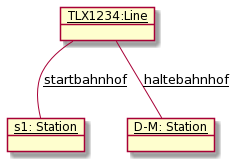
\includegraphics[width=0.45\textwidth]{./Aufgabe10_1a}
	\end{center}
	Objektdiagramm nach Schritt 9 im Sequenzdiagramm
	\begin{center}
		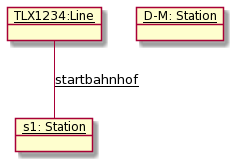
\includegraphics[width=0.45\textwidth]{./Aufgabe10_1b}
	\end{center}

	\section*{Aufgabe 2}
	Die Fehler sind
	\begin{itemize}
		\item Die Bahnlinie EC173 hat 2 Endbahnhöfe.
		\item Die Lok L1 kann nicht direkt einer Fahrt zugeordnet werden, sondern nur einem Zug, der einer Fahrt zugeordnet wird.
		\item Eine Fahrt kann nur einer Bahnlinie zugeordnet werden und nicht 2. (Fahrt 1 $\to$ S1-2, S1-1)
		\item VORFRISTIG ist kein gültiger Zustand; gültige Zustände wären PÜNKTLICH oder UNPÜNKTLICH.
		\item Die Bahnlinie S1-1 hat keinen Startbahnhof.
		\item Die Bahnlinie S1-2 hat keinen Endbahnhof.
		\item Der Bahnlinie EC173 ist keine Fahrt zugeordnet.
	\end{itemize}

	\section*{Aufgabe 3}
	\begin{center}
		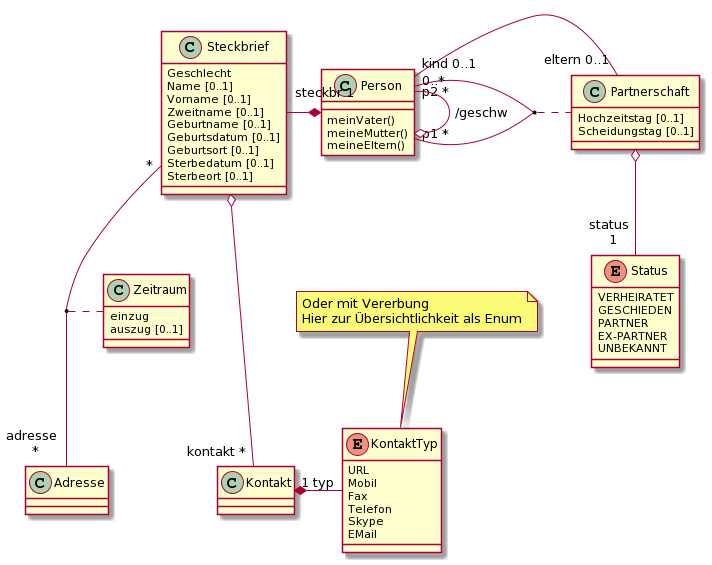
\includegraphics[width=1\textwidth]{./Aufgabe10_3}
	\end{center}
	
\end{document}